% =====================================================================
% A2 — Section 3: Reproduction protocol.  DRAFT 2, 3 Oct 2026.
% Restructured after the A1 feedback: each subsection opens with why it
% exists; the hyperparameter list moved to Table 1 (tables do not count
% towards the page limit). Every number checked against code and results.
% The brief requires model reductions to be stated: there are none (3.5).
% =====================================================================

\section{Reproduction protocol}
\label{sec:methods}

I begin by rerunning the authors' experiment exactly as released, to check
that their code reproduces their own saved results. Because C2 claims a
transition in the probability that a network finds the linear representation,
I then repeat the experiment with enough runs to estimate that probability at
each training data fraction.

% Fig. 2 (C1) defined here so it is placed before the wide Fig. 3;
% LaTeX keeps figures in order, so a late Fig. 2 would push Fig. 3 back a page.
\begin{figure}[t]
  \centering
  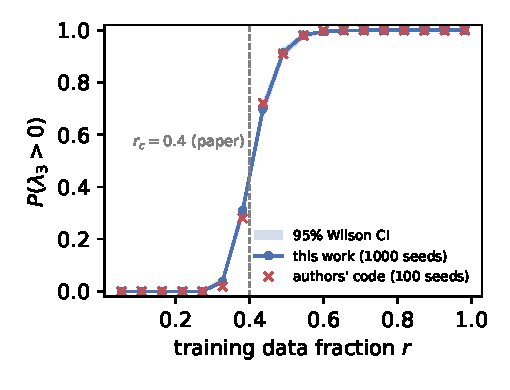
\includegraphics[width=\linewidth]{figures/fig4a}
  \caption{C1. Probability that a random training set determines the linear
  representation ($\lambda_3>0$) against the training data fraction. 1000 training
  sets per size (band: 95\% Wilson interval). Crosses: the authors' code on
  100 of the same training sets. Dashed: $r_c=0.4$ as stated in the paper.}
  \label{fig:c1}
\end{figure}

% Fig. 3 (two columns) defined here too: figure* floats to the next page,
% which puts it next to Sec. 4.
\begin{figure*}[t]
  \centering
  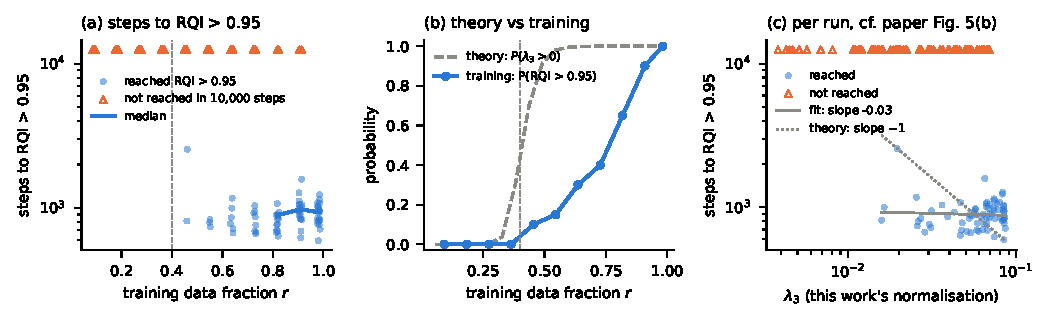
\includegraphics[width=\textwidth]{figures/fig4b_baseline}
  \caption{C2 and C3 with the released configuration, 20 seeds per size.
  (a)~Steps to $\mathrm{RQI}>0.95$. Triangles: runs that never reach it in
  $10^4$ steps. Line: median with failed runs counted as $\infty$.
  (b)~Fraction of runs reaching $\mathrm{RQI}>0.95$, against the theory's
  $\Pr(\lambda_3>0)$. (c)~Steps against $\lambda_3$ for every run with
  $\lambda_3>0$ (compare the paper's Fig.~5b). Grey: least-squares fit to the
  successful runs. Dotted: the slope $-1$ predicted by the theory.}
  \label{fig:c2}
\end{figure*}

\subsection{Code and configuration}
\label{sec:config}

All runs use the authors' released code~\cite{liu2022code} without any
modification, so that a discrepancy cannot come from a re-implementation. The
code is pinned at commit \texttt{0229df9} (November 2022) and run on CPU with
PyTorch~2.14.

The paper does not state the hyperparameters behind its own Fig.~4(b), and its
appendix gives only the decoder architecture and the embedding learning rate.
Instead, I use the settings of the released script that generates this
figure, listed in Table~\ref{tab:config}. The script trains three seeds per
training size. I train twenty, including the authors' three. One seed fixes
the targets, the training split, the initialisation and the order of
minibatches, giving 220 runs per configuration.

\begin{table}[t]
  \centering
  \caption{Training configuration of the released script, used for all
  runs. Ablations change one row at a time (marked $^{*}$).}
  \label{tab:config}
  \small
  \begin{tabular}{@{}ll@{}}
    \toprule
    Decoder & MLP 1--200--200--30, $\tanh$ \\
    Embeddings & $d_{\mathrm{in}} = 1$, initialised $\mathcal{U}(-\tfrac12, \tfrac12)$ \\
    Targets $\mathbf{Y}_c$ & $\mathcal{N}(\mathbf{0}, \mathbf{I})$ in $\mathbb{R}^{30}$, squared-error loss \\
    Optimiser & AdamW~\cite{loshchilov2019decoupled} for both parts \\
    Learning rates & embeddings $10^{-3}$, decoder$^{*}$ $10^{-4}$ \\
    Weight decay & none$^{*}$ \\
    Minibatch & $\min(45, |D|)$ training pairs \\
    Budget & $10^4$ steps \\
    Training sizes & $|D| \in \{5, 10, \dots, 50, 54\}$ ($r = 0.09$--$0.98$) \\
    Seeds & 0--19 per size (released script: 0--2) \\
    \bottomrule
  \end{tabular}
\end{table}

\subsection{Measurements}
\label{sec:measure}

For each run, the question is to see whether and when it finds the linear representation, and how this compares with what the theory predicts for its training set.

\emph{Steps to $\mathrm{RQI} > 0.95$.} RQI is computed at every step as in
the released code, on normalised embeddings and with tolerance $\delta = 0.1$.
As in the paper, I record the number of steps until $\mathrm{RQI} > 0.95$.
At each training size I also record the fraction of runs that get there
within $10^4$ steps, and where this fraction passes one half.

\emph{Runs that do not succeed.} The released code reports
the last step for these runs, which cannot be told
apart from a run that succeeds exactly at the end. I therefore have chosen to record success separately, treat unsuccessful runs as infinitely slow when taking
medians, and leave the median undefined if more than half the runs at a size
fail.

\emph{Theory.} I computed $\lambda_3$ with my own implementation of
\eqref{eq:hessian}, independent of the authors' code. For C1, $\Pr(\lambda_3 > 0)$ is estimated from 1000 random training sets per training size, and for C3, $\lambda_3$ is computed for the training set of every trained run.

I set $Z_0 = p$, its value for unit-variance embeddings. As a result, my $\lambda_3$ differs from the paper's by a constant factor, which is why it is compared only through ranks and slopes.

\subsection{Statistical analysis}
\label{sec:stats}

Every configuration is trained on the same 220 training sets. Runs with the
same seed are not independent, since across sizes they share targets,
initialisation, and nested training sets. Configurations are therefore compared seed by seed, and I count the seeds whose number of successes with
$\lambda_3 > 0$ goes up or down, and use an exact sign test.

Within one training size the seeds are independent, so success probabilities
there are given with Wilson 95\% intervals~\cite{wilson1927probable}. For C3,
Spearman's $\rho$ and the log--log slope (theory: $-1$) are only descriptive,
because $\lambda_3$ also grows with the training size.

\subsection{Ablations}
\label{sec:ablations-setup}

The ablations test which part of training decides whether a determined
representation is actually found. Each repeats all 220 runs with one setting
changed, either \textbf{(A1)} decoder weight decay of 1 or 5, or \textbf{(A2)} a
decoder learning rate of $10^{-5}$ or $10^{-3}$. Both are axes of the paper's
own phase diagrams, which describe a competition between representation
learning and the decoder. I also retrain samples of unsuccessful runs with $\lambda_3 > 0$ for $5 \times 10^4$ steps, to tell slow runs from stuck ones.

\subsection{Deviations from the original study}
\label{sec:deviations}

I use the paper's model, task and training procedure. No smaller or
modified model is used. The study deviates in four documented ways, here twenty seeds
instead of three, the released configuration in place of the
undocumented settings of the published Fig.~4(b), $\lambda_3$ known up
to a constant factor, and handling of runs that never succeed.
